\documentclass[handout]{beamer}
%\documentclass [serif,mathserif,professionalfont]{beamer}
%\usepackage {pxfonts}
%\usepackage {eulervm}
%\usepackage{mathpazo}
%\logo{\includegraphics[height=1.2cm]{fsulogo.png}}

\usepackage{tikz}
\usepackage{graphicx}
\usepackage{subfig,fixltx2e,url}
\usepackage[latin1]{inputenc}
\usepackage{pgfplots}
\usepackage{subcaption}
\usepackage{hyperref}

%\usetheme{Warsaw}
\usecolortheme{lily}
\setbeamercovered{transparent}
%\useoutertheme[subsection=false]{smoothbars}

\setbeamertemplate{sidebar right}{}
\setbeamertemplate{footline}{%
\hfill\usebeamertemplate***{navigation symbols}
\hspace{1cm}\insertframenumber{}/\inserttotalframenumber}

\title[ \insertdate]{Multi-Input Multi-Output Electric Motor Signal Prediction using Neural Networks}

\author{Sagar Verma}
\institute[Centralesup\'elec and Schneider Electric] % (optional, but mostly needed)
{
  Centre de Vision Num\'erique,\\
  Centralesup\'elec, Gif-sur-Yvette}
% - Use the \inst command only if there are several affiliations.
% - Keep it simple, no one is interested in your street address.

\date{November, 2018}
% - Either use conference name or its abbreviation.
% - Not really informative to the audience, more for people (including

\begin{document}

\begin{frame}
\titlepage
\end{frame}

\section{Problem Statement}

\begin{frame}{Problem Statement}
\begin{center}
\begin{enumerate}
  \item Input: multiple signals
  \item Output: multiple signals.
  \item Continuous signals: regression problem.
\end{enumerate}
\vspace{.5cm}
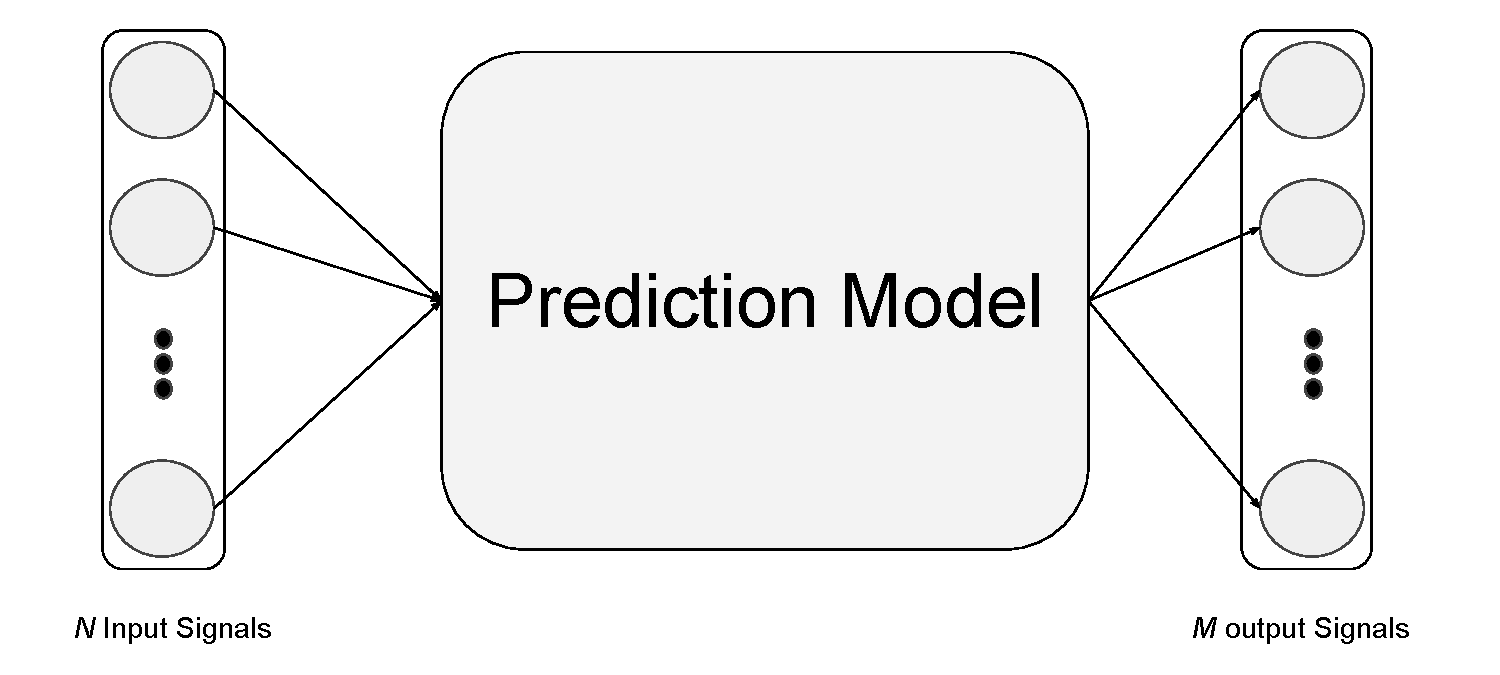
\includegraphics[width=1\linewidth]{images/teaser}
\end{center}
\end{frame}


\begin{frame}{Challenges}
  \begin{enumerate}
    \item How to handle continous signals?
    \item How to handle long sequences? Electric motors generally operate for long hours.
    \item Which prediction model to use?
    \item How to handle multiple outputs?
  \end{enumerate}
\end{frame}

\section{Background}
\begin{frame}{Background}
  \begin{enumerate}
    \item Perceptrons
    \item Feed-forward Networks
    \item Activation Functions
    \item Backpropagation
    \item Loss Functions
    \item Sequential Networks
    % \item Generative Networks
  \end{enumerate}
\end{frame}

\begin{frame}{Perceptrons}
\begin{enumerate}
  \item Basic block of neural networks \\

  \item Input: binary variables, $x_i$ \\

  \item Output: Binary decision, $y$ \\

  \item $w_i$ is a weight, output is calculated using \\

  \begin{eqnarray}
  \mbox{output} & = & \left\{ \begin{array}{ll}
      0 & \mbox{if } \sum_i w_i x_i \leq \mbox{ threshold} \\
      1 & \mbox{if } \sum_i w_i x_i > \mbox{ threshold}
      \end{array} \right.
\tag{1}\end{eqnarray}
\end{enumerate}
    \begin{center}
      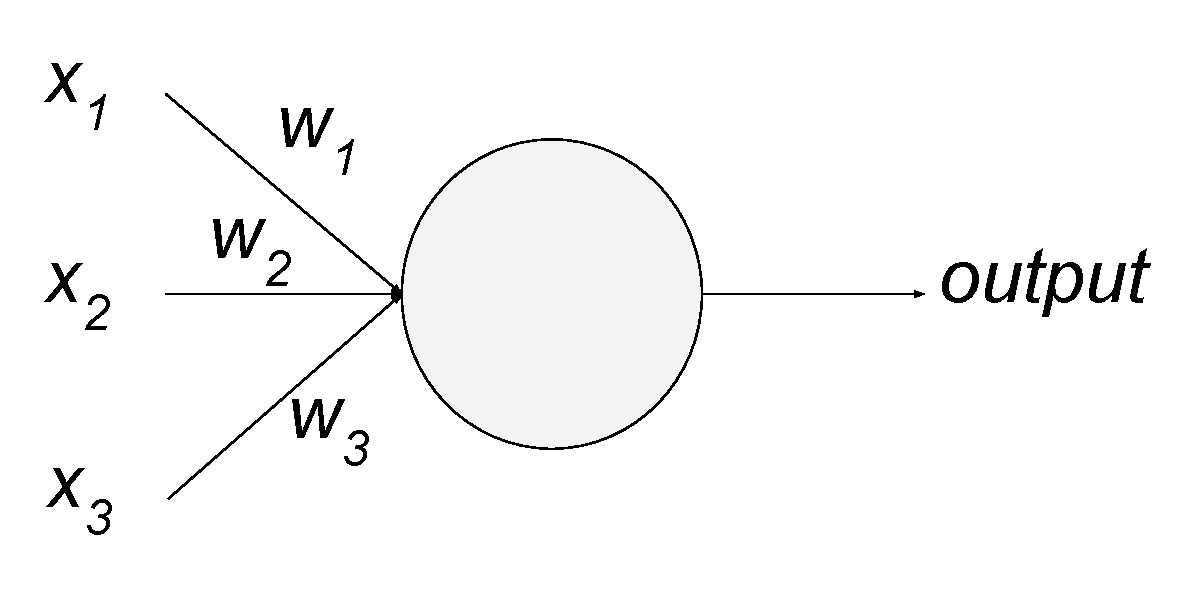
\includegraphics[width=0.8\linewidth, height=4cm]{images/perceptron}
    \end{center}
\end{frame}

\begin{frame}{Feed-forword Networks}
\begin{enumerate}
  \item AKA Artificial Neural Networks (ANNs) \\

  \item Multiple stacked perceptrons \\

  \item \#connections increases with \#perceptrons, input size, and output size \\

  \item Learning weights is difficult
    \begin{enumerate}
      \item Binary output does not tell us which weights are important and which are not \\
      \item A small change in input or weight could flip the output from 0 to 1 or vice versa \\
    \end{enumerate}
\end{enumerate}
    \begin{center}
      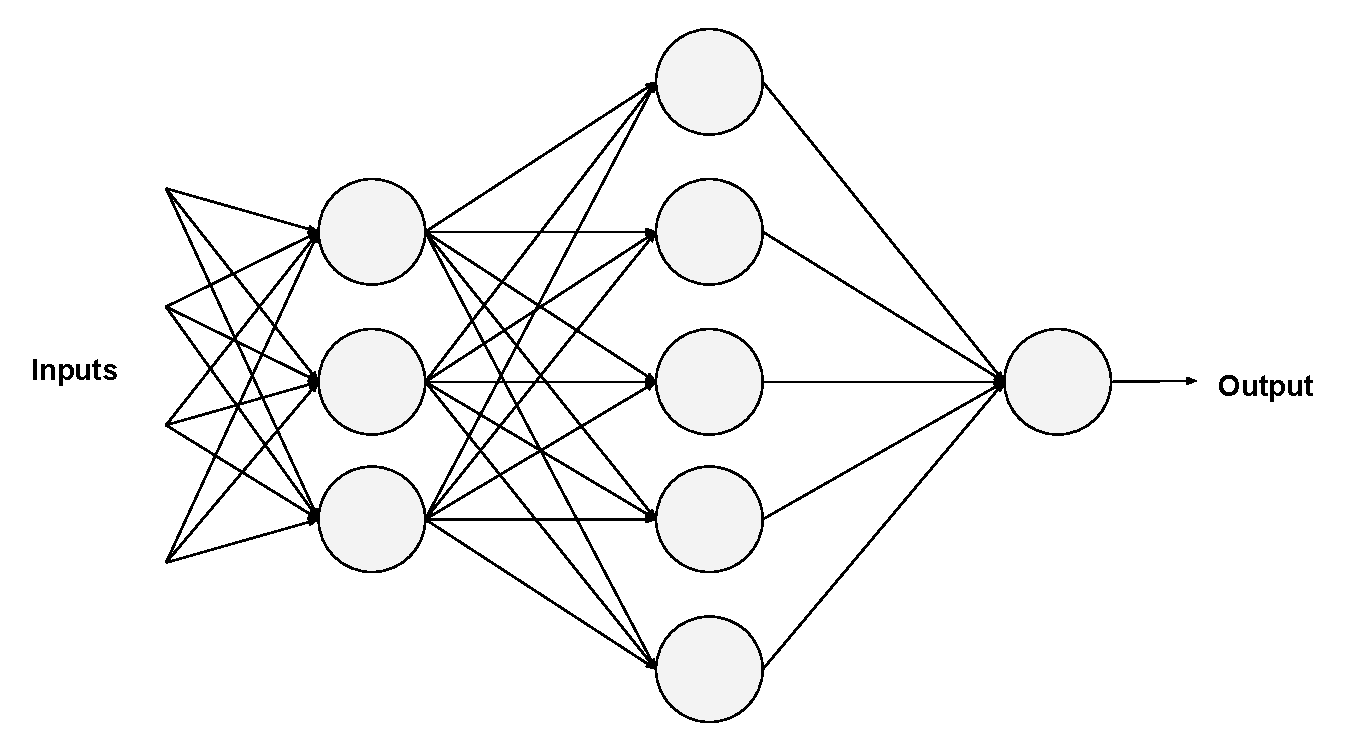
\includegraphics[width=0.65\linewidth, height=3.5cm]{images/anns}
    \end{center}
\end{frame}

\begin{frame}{Activation Functions}
  \begin{enumerate}
    \item To learn weights of an ANN we need continous output. \\

    \item Function that can give small changes in output when small changes in weights are made. \\

    \item Should give a smooth output. \\

    \item $f$ should be non-linear, $y = f(w^Tx+b)$ \\
  \end{enumerate}
  \begin{center}
    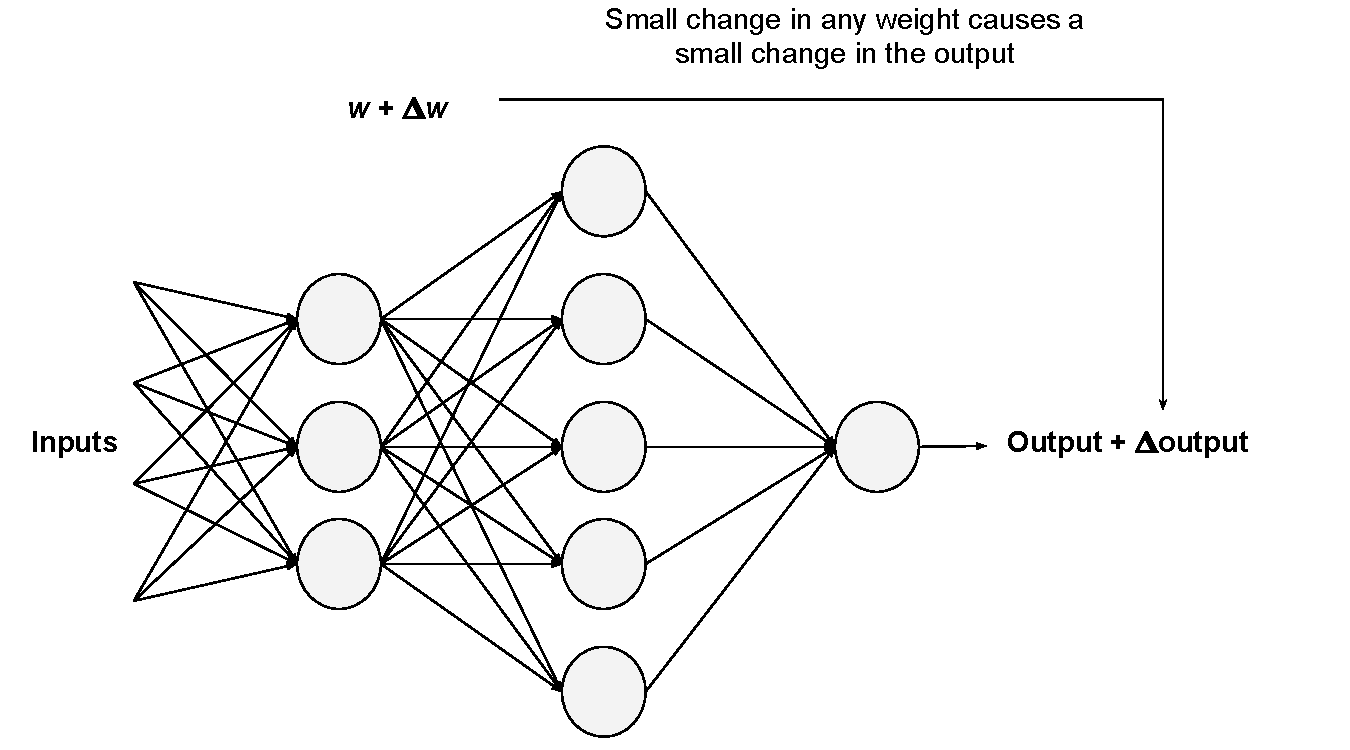
\includegraphics[width=0.65\linewidth, height=3.5cm]{images/anns_change}
  \end{center}
\end{frame}

\begin{frame}{Activation Functions: Examples}


\begin{enumerate}

  \item Sigmoid: $ f(x) = \sigma(x) = \frac{1}{1+\exp(-\sum_i w_i x_i)}$ \\

  \item Tanh: $ f(x) = tanh(x) = \frac{\exp(\sum_i w_i x_i) - \exp(-\sum_i w_i x_i)}{\exp(\sum_i w_i x_i) + \exp(-\sum_i w_i x_i)}$ \\

  \item Rectified Linear Unit (ReLU): $f(x) = \left\{\begin{array}{ll}
      0 & \mbox{if } \sum_i w_i x_i < \mbox{ 0} \\
      x & \mbox{if } \sum_i w_i x_i \geq \mbox{ 0}
      \end{array}$ \\
\end{enumerate}

\vspace{0.5cm}

\begin{center}
      \resizebox{2cm}{2cm}{
        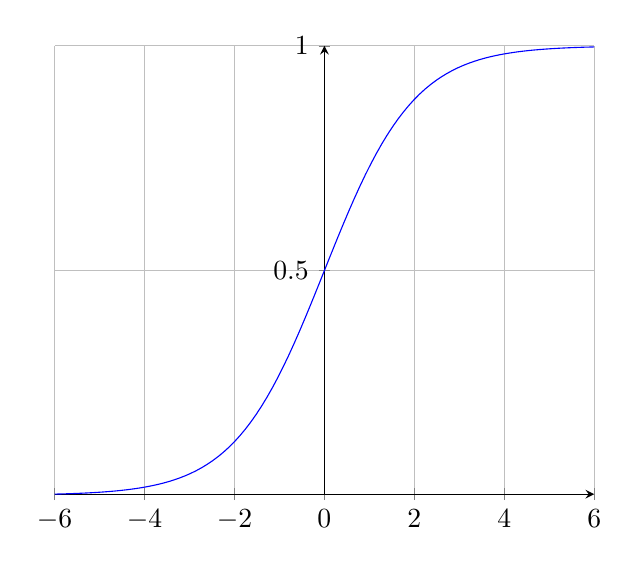
\begin{tikzpicture}
          \begin{axis}%
          [
              grid=major,
              xmin=-6,
              xmax=6,
              axis x line=bottom,
              ytick={0,.5,1},
              ymax=1,
              axis y line=middle,
          ]
              \addplot%
              [
                  blue,%
                  mark=none,
                  samples=100,
                  domain=-6:6,
              ]
              (x,{1/(1+exp(-x))});
          \end{axis}
        \end{tikzpicture}}
      \resizebox{2cm}{2cm}{
        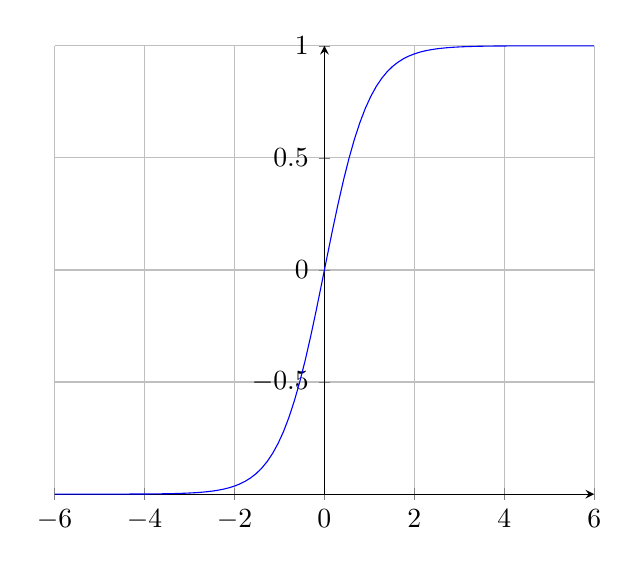
\begin{tikzpicture}
          \begin{axis}%
          [
              grid=major,
              xmin=-6,
              xmax=6,
              axis x line=bottom,
              ytick={-.5,0,.5,1},
              ymax=1,
              axis y line=middle,
          ]
              \addplot%
              [
                  blue,%
                  mark=none,
                  samples=100,
                  domain=-6:6,
              ]
              (x,{(exp(x)-exp(-x))/(exp(x)+exp(-x))});
          \end{axis}
        \end{tikzpicture}}
      \resizebox{2cm}{2cm}{
        \begin{tikzpicture}
          \begin{axis}%
          [
              grid=major,
              xmin=-6,
              xmax=6,
              axis x line=bottom,
              ytick={-5,1,2,3,4,5},
              ymax=5,
              axis y line=middle,
          ]
              \addplot%
              [
                  blue,%
                  mark=none,
                  samples=100,
                  domain=-6:6,
              ]
              (x, ifthenelse(x<=0,0,x));
          \end{axis}
        \end{tikzpicture}}
\end{center}
\end{frame}


\begin{frame}{Loss Functions}
\begin{enumerate}
  \item Tells us how good or bad weights are. \\

  \item \textbf{L1 Loss} $\mathcal{L}(y_{true},y_{pred}) = |y_{true}-y_{pred}|$ \\

  \item \textbf{MSE Loss} $\mathcal{L}(y_{true},y_{pred}) = (y_{true}-y_{pred})^2$ \\

  \item \textbf{Cross Entropy Loss} (classification) $\mathcal{L}(y_{true},y_{pred}) = -\sum_{c=1}^{C}y^c_{true}log(y^c_{pred})$ \\
\end{enumerate}
\end{frame}

\begin{frame}{}
    \center
    \Large{\color{blue}We have a network (ANN + activation function). \\
    We can judge it (loss function). \\
    \textit{How do we learn weights?}}
\end{frame}

\begin{frame}{Learning Weights}
  \begin{enumerate}
    \item Small loss means good weights.
    \item Learn weights using \textit{Optimizers}.
  \end{enumerate}
\end{frame}

% \begin{frame}{Backpropagation}
%   \begin{enumerate}
%     \item Forward propogate input to get output from a network.
%     \item Calculate loss.
%     \item Backpropagate the loss(error) to all the weights.
%     \item Each weight's output and input activation are mutliplied to find the gradient of the weight.
%     \item A ratio of the weight's gradient is subtracted from the weight.
%   \end{enumerate}
% \end{frame}

\begin{frame}{Optimizers}
  \begin{enumerate}
    \item Cannont process large dataset at once.
    \item Process data in small parts (mini-batches).
    \item Optimizers for learning weights using mini-batches.
    \item Stochastic Gradient Descent is the most used optimizer.
  \end{enumerate}
\end{frame}

\begin{frame}{}
  \center
  \Large{\color{blue}We can now train an ANN. \\
  Can we process continous signals?}
\end{frame}

\begin{frame}{Sequential Networks}
  \begin{enumerate}
    \item ANNs can be used by splitting sequences.
    \item Sequence networks for temporal learning.
    \item Recurrent neural networks (RNNs) and Long-Short Term Memorry (LSTM).
  \end{enumerate}
  \begin{center}
    \begin{figure}
    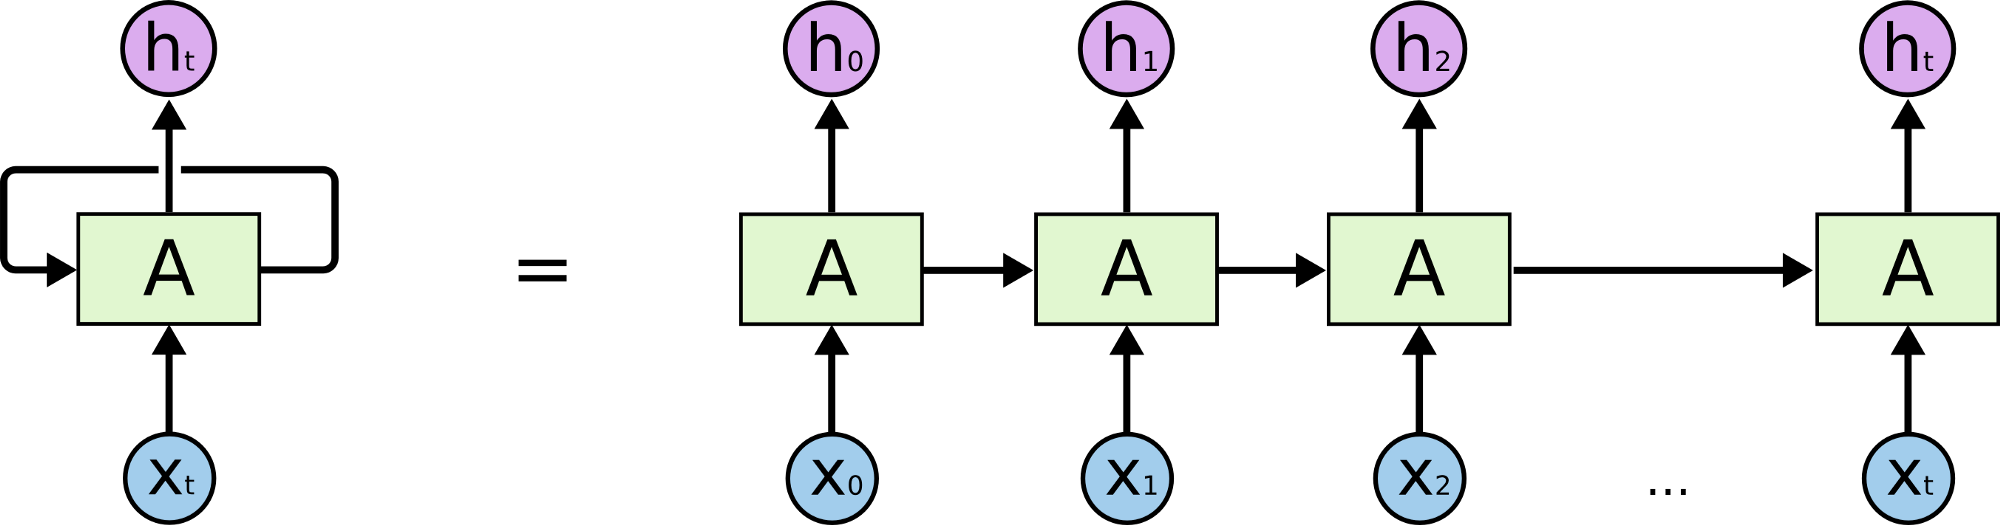
\includegraphics[width=0.65\linewidth, height=2cm]{images/rnn}
    \caption{RNN unrolled in time. \href{https://towardsdatascience.com/introduction-to-recurrent-neural-network-27202c3945f3}{\color{blue}\textit{source}}}
    \end{figure}
  \end{center}
\end{frame}

\begin{frame}{Recurrent Neural Networks}
  \begin{enumerate}
    \item Perform same task for every element of a sequence.
    \item Output depends on previous elements.
    \item RNNs can be seen as a neural network having "memory".
    \begin{equation}
        h_t = tanh(Wx_t+Uh_{t-1}),
    \end{equation}
    where $W$ and $U$ are weights, $h$ is the hidden vector and $x_t$ is the input at time $t$.
  \end{enumerate}

\end{frame}

\begin{frame}{Long-Short Term Memory}
  \begin{enumerate}
    \item RNNs have vanishing and exploding gradients problem.
    \item In practice gradients become too big or small for long sequences.
    \item LSTM resolves above problems.
    \item Knows when to forget and when to remember.
    % \begin{center}
    %   \begin{figure}
    %   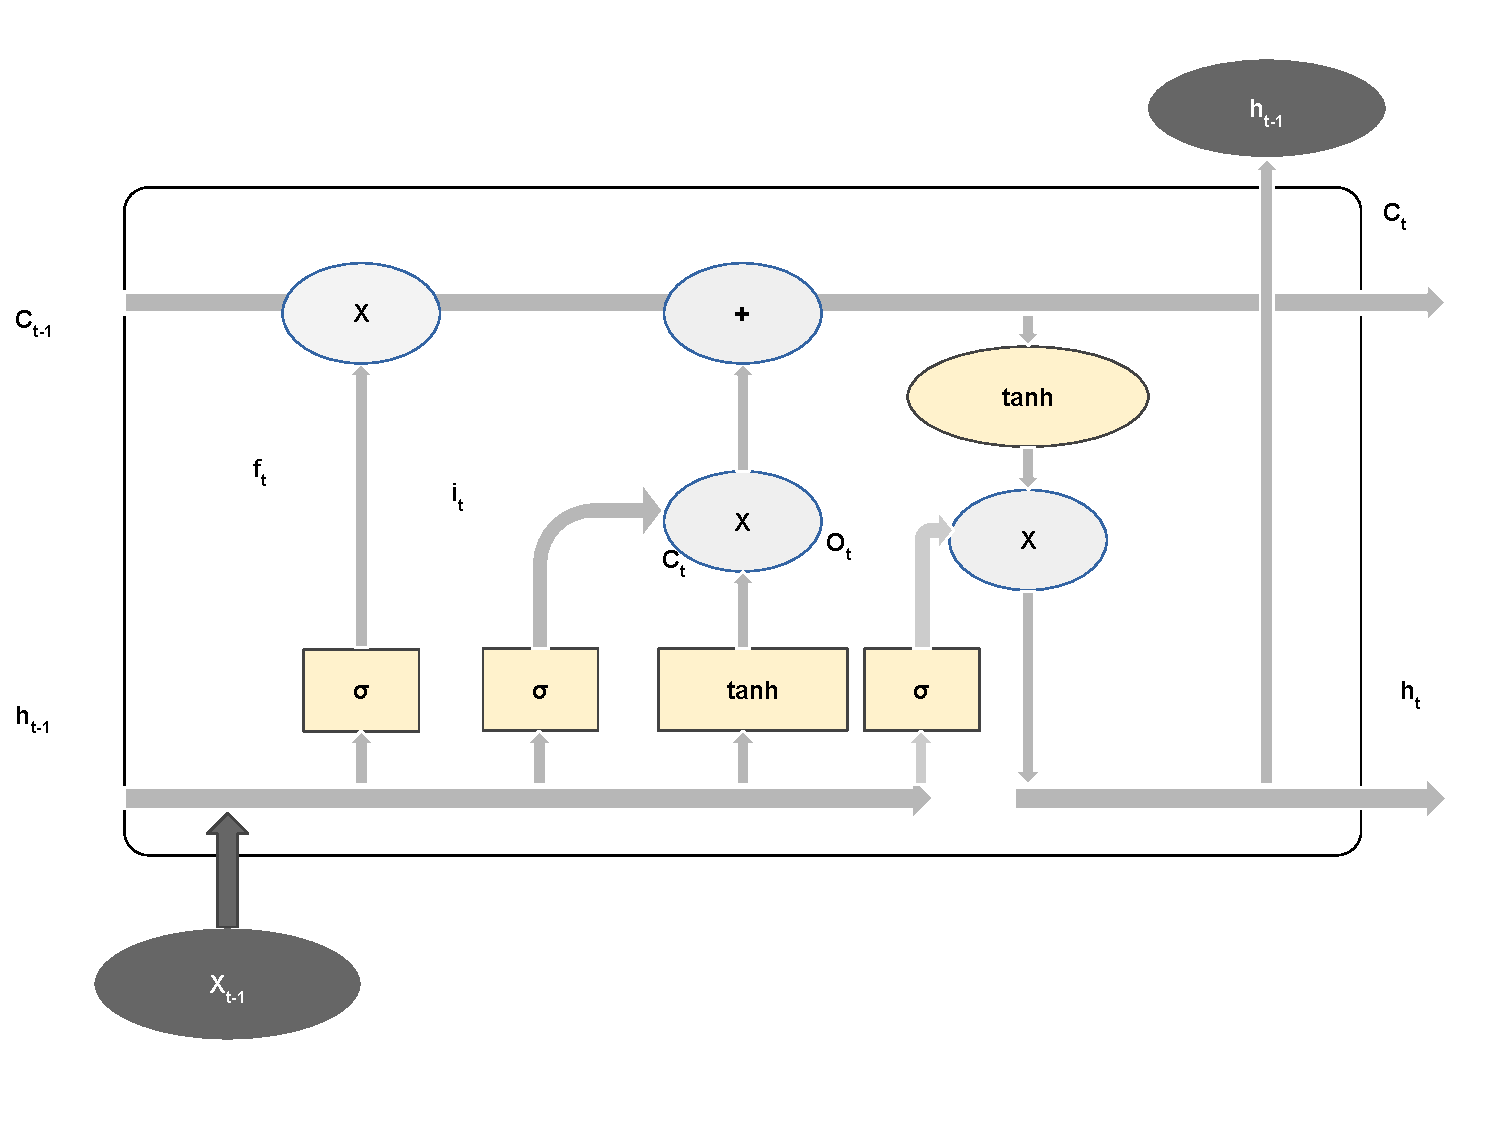
\includegraphics[width=0.6\linewidth, height=4cm]{images/lstm}
    %   \caption{LSTM Cell.}
    %   \end{figure}
    % \end{center}
  \end{enumerate}
\end{frame}

% \begin{frame}{Generative Networks}
%   \begin{enumerate}
%
%   \end{enumerate}
% \end{frame}

\begin{frame}{}
  \center\Large{\color{blue}Neural networks for motor control}
\end{frame}

\section{Dataset}
\begin{frame}{Dataset}
  \begin{enumerate}
    \item \textit{CNC Mill Tool Wear} dataset from \href{https://www.kaggle.com/shasun/tool-wear-detection-in-cnc-mill}{\color{blue}\textit{kaggle}}.
    \item Provides real world motor speed.
    \item 18 experiments under different conditions.
    \item Mean experiment time is 136.6389 seconds.
    \item 14 experiments are used for training and 4 for testing.
  \end{enumerate}
\end{frame}

\section{Experiments and Results}
\begin{frame}{Experimental Setup}
  \begin{enumerate}
    \item Simulink model generates voltages, currents and torque.
    \item PyTorch for network implementation.
    \item Dataset scaled between $(-1,1)$.
    \item Simulink gives data at 20KHz, downsample to 100Hz.
    \item Splitting data, window size: 60 at stride: 10.
    \item Mean Square Error (MSE) to evaluate.
  \end{enumerate}
\end{frame}

\begin{frame}{ANN for signal prediction}
  \begin{enumerate}
    \item Three outputs, three networks.
    \item Input: $180, 60\times3$
    \item Output: $60$
    \item Architecture: 3 Layers, 180x360 -> 360x120 -> 120X60
    \item Current1 model MSE: 0.043
    \item Current2 model MSE: 0.105
    \item Torque model MSE: 0.564
  \end{enumerate}
  \begin{table}[]
    \begin{tabular}{c c c}
     Model & Current1 & Current2 & Torque\\
     MSE & 
    \end{tabular}
    \end{table}
\end{frame}

\begin{frame}{LSTM for signal prediction}
  \item Three outputs, three networks.
  \item Input: $60\times3$
  \item Output: $60$
  \item Current1 model MSE: 0.043
  \item Current2 model MSE: 0.105
  \item Torque model MSE: 0.564
\end{frame}

% \begin{frame}{RBM for signal prediction}
%
% \end{frame}

\begin{frame}{Multiple models or Single model?}

\end{frame}

\section{Conclusions and Future Work}
\begin{frame}{Conclusions}

\end{frame}

\begin{frame}
\huge{Thank you}\\
\huge{Questions?}\\
\end{frame}

\end{document}
